% Sprinkler pumpe system

\subsection{Sprinkler-pumpe system ()}

Sprinkleren skal forsynes med et vandtryk fra en vandpumpe. Grundfos har doneret en Alpha2 pumpe til formålet. Alpha2 pumpen kræver 230 VAC. Det overskrider hvad der dagligt må arbejde med for studerende på AU. Der er derfor efter aftale med Torben Lund Jensen fra værkstedet givet særskilt tilladelse til at designe og implementere et lukket 230 V / 5 V relæ. Figur \ref{lab:Relay_box} viser kredsløbet for det lukkede 230 V / 5 V relæ. Jordforbindelsen løber direkte igennem og er altid forbundet, mens fasen og nul forbindes/afbrydes af relæet.  

\begin{figure}[H]
  \centering
    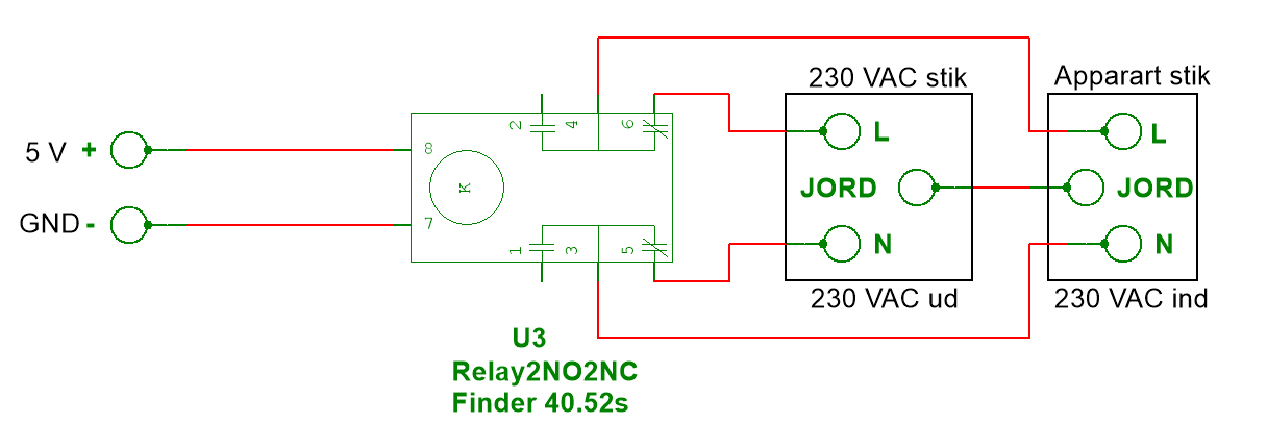
\includegraphics[width=0.75\textwidth]{Billeder/230VAC_KREDS}
    \caption{Kredsløbsdiagram for lukket 230 V / 5 V relæ}
    \label{lab:Relay_box}
\end{figure}